\documentclass{standalone}
% \documentclass{article}

\usepackage{tikz}

\begin{document}

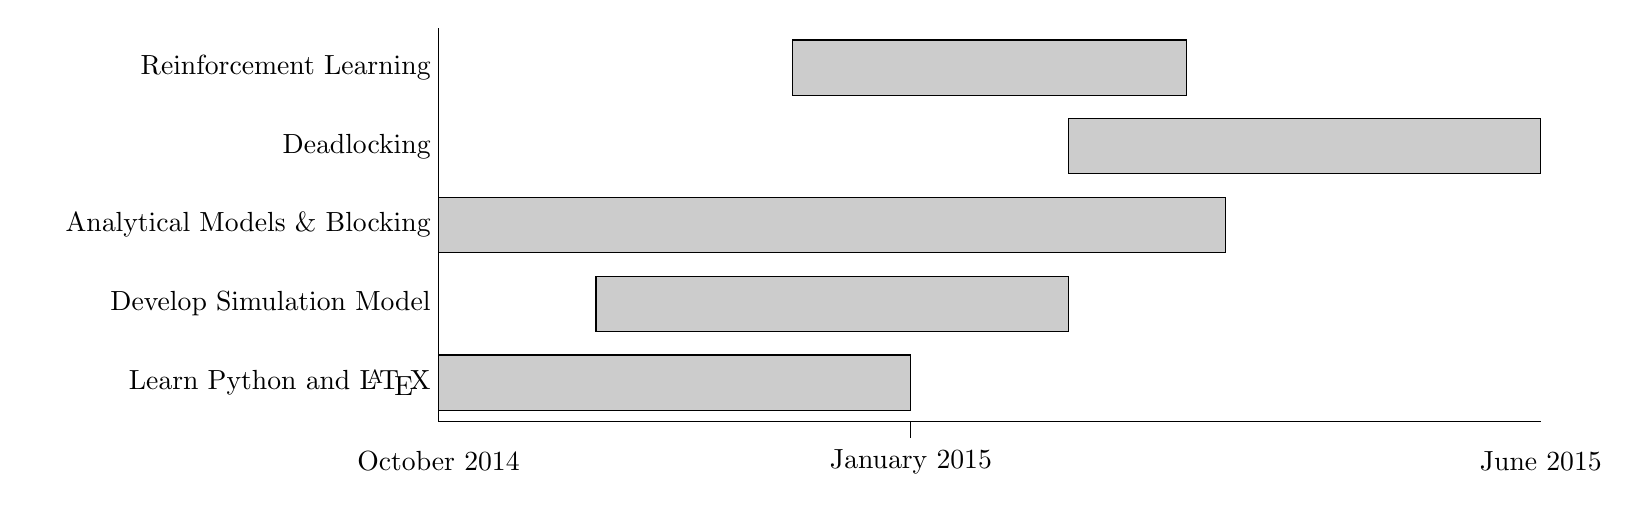
\begin{tikzpicture}

\draw (0, 5) -- (0, 0);
\draw (0, 0) -- (14, 0);
\draw (6, 0) -- (6, -0.2);

\draw [draw=black,fill=black!20] (0, 0.15) rectangle (6, 0.85);
\draw [draw=black,fill=black!20] (2, 1.15) rectangle (8, 1.85);
\draw [draw=black,fill=black!20] (0, 2.15) rectangle (10, 2.85);
\draw [draw=black,fill=black!20] (8, 3.15) rectangle (14, 3.85);
\draw [draw=black,fill=black!20] (4.5, 4.15) rectangle (9.5, 4.85);

\node at (6, -0.5) {January 2015};
\node at (0, -0.5) {October 2014};
\node at (14, -0.5) {June 2015};

\node[align=right,text width=5cm] at (-2.6, 0.5) {Learn Python and \LaTeX};
\node[align=right,text width=5cm] at (-2.6, 1.5) {Develop Simulation Model};
\node[align=right,text width=5cm] at (-2.6, 2.5) {Analytical Models \& Blocking};
\node[align=right,text width=5cm] at (-2.6, 3.5) {Deadlocking};
\node[align=right,text width=5cm] at (-2.6, 4.5) {Reinforcement Learning};

\end{tikzpicture}

\end{document}
